\chapter{Methodology}
\label{ch:method}

\section{Overview}

The system has three parts (\cref{fig:pipeline}). A frozen ImageNet-pretrained CNN turns each image
into an embedding. A small trainable adapter inside the backbone changes those embeddings; it is the
only part that is trained, apart from two scalars in the evidential head. A parameter-free prototype
head then classifies each query by its similarity to the class prototypes of the current episode, and
the resulting logits are read either as a softmax or as Dirichlet evidence.

\begin{figure}[H]
\centering
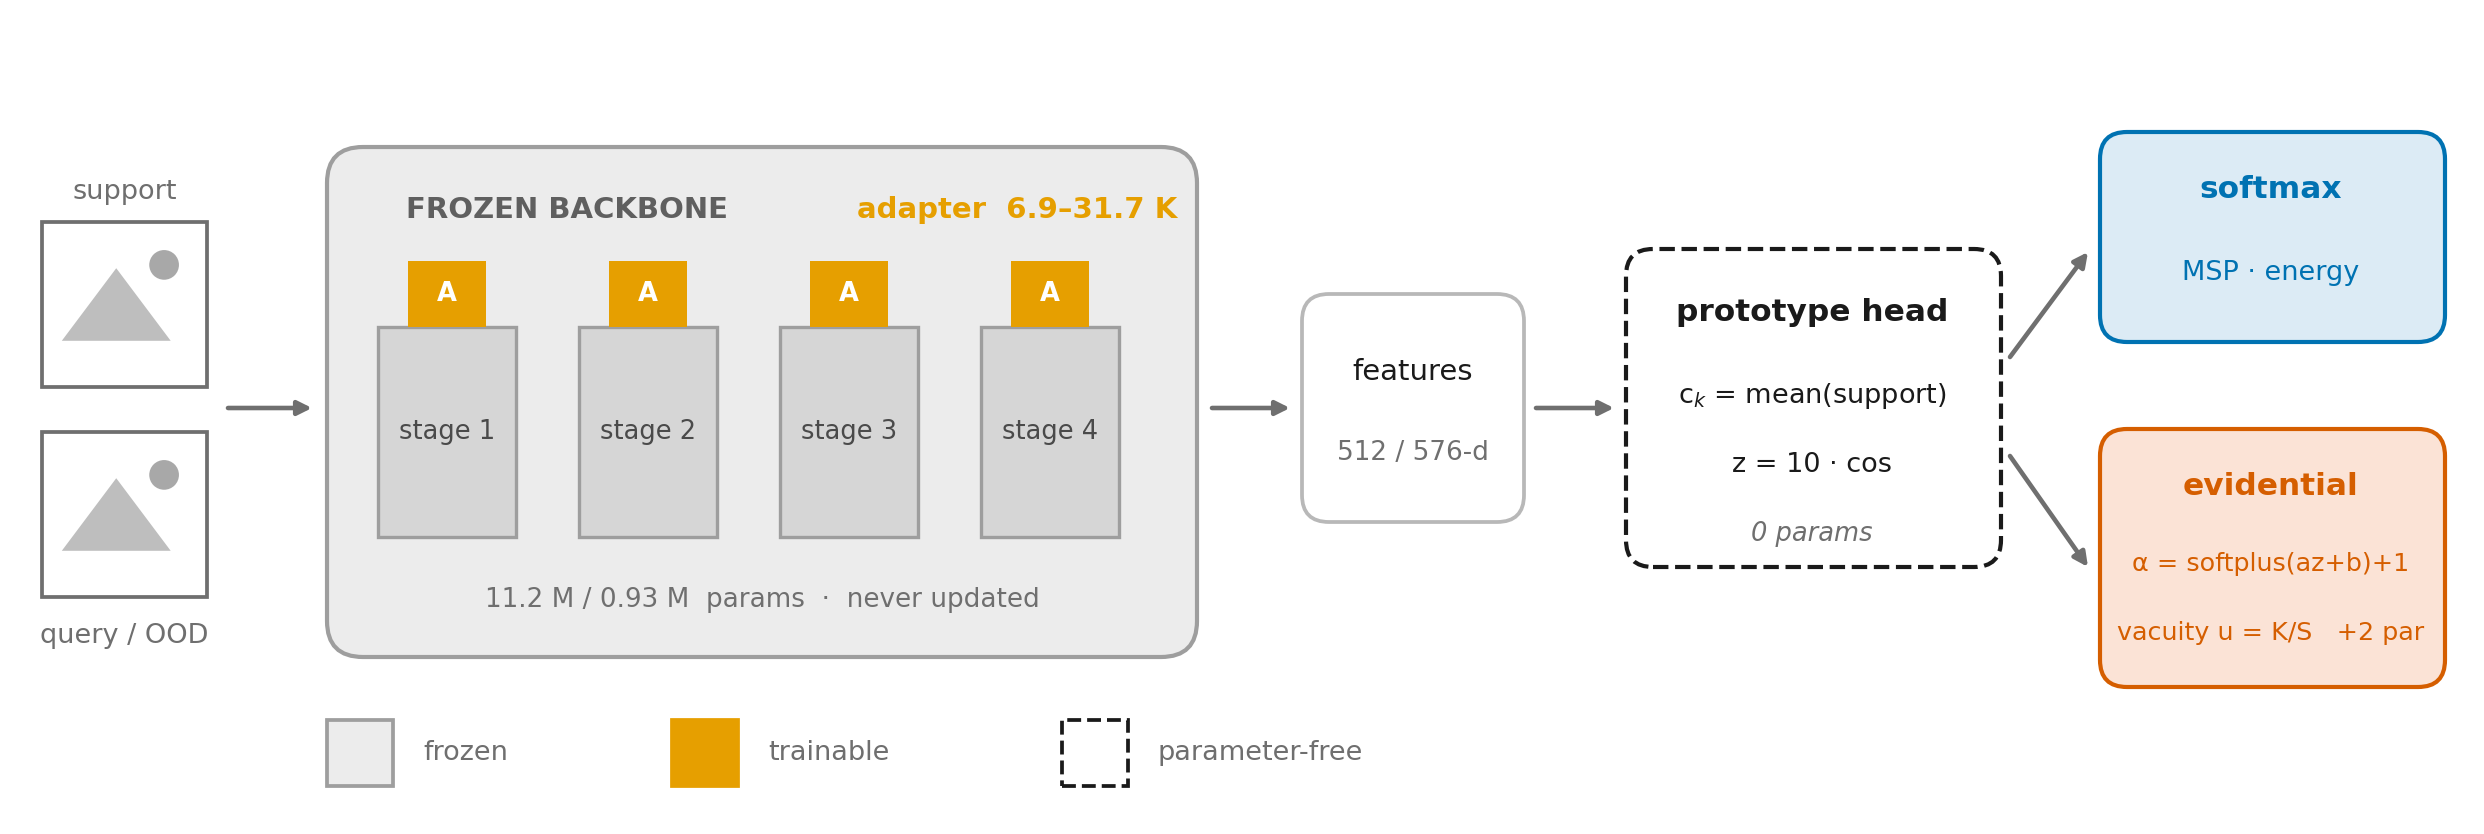
\includegraphics[width=\textwidth]{F4_architecture_pipeline.png}
\caption{The pipeline. Support and query images pass through the frozen backbone with a small trainable
adapter. The features feed a parameter-free prototype head whose logits are read as softmax
probabilities or as evidential (Dirichlet) evidence. Only the adapter and, for the evidential head, two
evidence parameters are trained.}
\label{fig:pipeline}
\end{figure}

\section{Adapters}
\label{sec:adapters}

Two adapter designs form the main comparison (\cref{fig:adapters}). Both are initialised so that the
adapted network starts out identical to the pretrained one.

\begin{figure}[H]
\centering
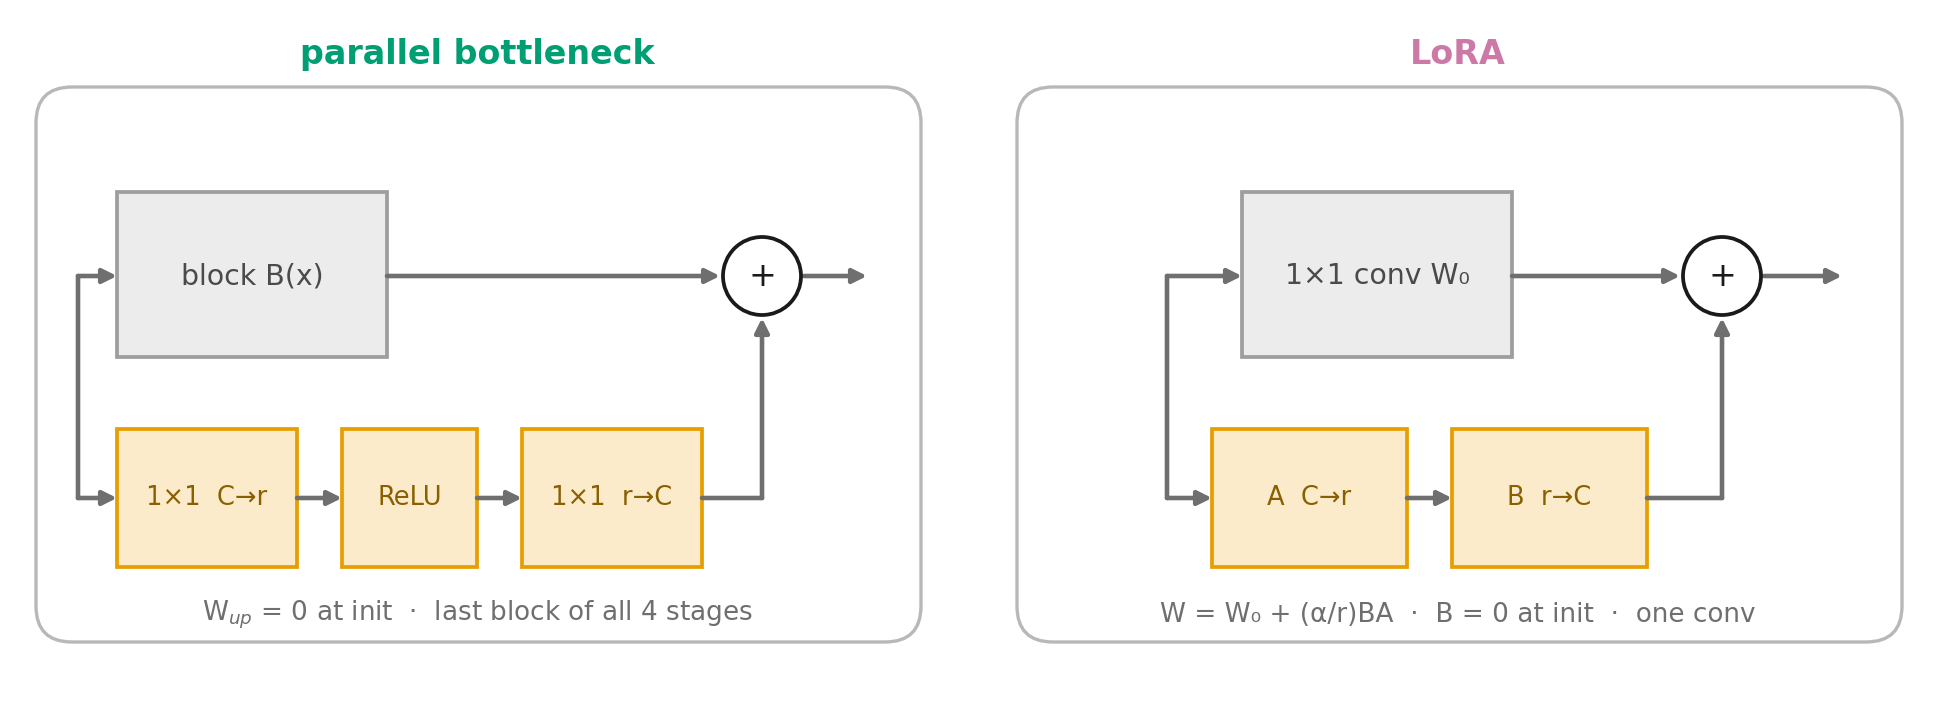
\includegraphics[width=0.95\textwidth]{F5a_adapter_zooms.png}
\caption{The two adapter designs. Left: the parallel bottleneck, a side branch added at the last block
of each of the four stages. Right: LoRA, a low-rank update inside one frozen $1\times1$ convolution.}
\label{fig:adapters}
\end{figure}

\paragraph{Parallel bottleneck adapter.} Following Houlsby et al.~\cite{houlsby2019adapters}, the
adapter is a down-projection to $r$ channels, a ReLU and an up-projection back to $C$ channels:
\begin{equation}
g(x) = W_{\text{up}}\, \mathrm{ReLU}(W_{\text{down}} x), \qquad W_{\text{down}} \in \mathbb{R}^{r \times C},\;
W_{\text{up}} \in \mathbb{R}^{C \times r}.
\end{equation}
Both projections are $1 \times 1$ convolutions with biases, applied at every spatial position, and
$W_{\text{up}}$ starts at zero. In the terminology of He et al.~\cite{he2022unified} the adapter is
\emph{parallel}: for the last block $B$ of each stage, the output becomes $B(x) + g(x)$, so the adapter
reads the block's input and its output is added to the block's output. One adapter is placed in each of
the four stages of ResNet-18, and in the last residual block of each of the four channel widths of
MobileNetV3-Small. We use $r = 16$. With biases, one stage costs $33C + 16$ parameters, which gives
31,744 parameters for ResNet-18 (stage widths 64, 128, 256, 512) and 6,928 for MobileNetV3-Small (stage
widths 24, 40, 48, 96). Because $1\times1$ convolutions mix channels but not neighbouring positions,
this adapter does not follow Conv-Adapter's advice to use spatial kernels~\cite{chen2024convadapter}; we
kept the simpler form so that the same adapter could be used unchanged on both backbones.

\paragraph{LoRA.} Following Hu et al.~\cite{hu2022lora}, LoRA adds a low-rank update to one frozen
$1 \times 1$ convolution:
\begin{equation}
W = W_0 + \tfrac{\alpha}{r}\, B A, \qquad A \in \mathbb{R}^{r \times C_{\text{in}}},\; B \in
\mathbb{R}^{C_{\text{out}} \times r},
\end{equation}
with $B$ initialised to zero, $r = 16$ and $\alpha = r$. On ResNet-18 the target is the $1\times1$
downsampling convolution at the start of the last stage ($256 \to 512$ channels), giving
$16 \times (256 + 512) = 12{,}288$ parameters. On MobileNetV3-Small it is the $1\times1$ projection
convolution of the deepest block ($576 \to 96$), giving 10,752 parameters. Applying LoRA to
convolutions follows earlier convolutional LoRA work~\cite{aleem2024convlora,zhong2024convlora}.

\paragraph{Baselines.} Two reference points are trained on ResNet-18 and CIFAR-FS only. \emph{Full
fine-tuning} unfreezes all 11.18M backbone parameters (learning rate $10^{-5}$, weight decay $10^{-4}$).
The \emph{linear probe} trains no backbone or adapter parameters: frozen features go straight to the
prototype head, so it has zero trainable parameters with the softmax head and only the two evidence
parameters with the evidential head.

\section{The Prototype Head}
\label{sec:head}

Classification uses a prototypical-network head~\cite{snell2017protonet}. For each of the $N$ classes of
an episode, the prototype is the mean embedding of its $K$ support images,
\begin{equation}
c_n = \frac{1}{K}\sum_{i \in \mathcal{S}_n} f_\theta(x_i),
\end{equation}
where $f_\theta$ is the frozen backbone with its adapter. A query $x$ receives one logit per class, its
scaled cosine similarity to that class's prototype:
\begin{equation}
z_n(x) = \tau \, \frac{f_\theta(x) \cdot c_n}{\lVert f_\theta(x)\rVert\, \lVert c_n \rVert}, \qquad \tau = 10 .
\label{eq:logits}
\end{equation}
The head has no trainable weights. This matters because the test classes are disjoint from the training
classes: a linear classifier trained on the 64 training classes has no outputs for the 20 test classes,
whereas prototypes can be computed for any class from its support images. At test time no gradient steps
are taken at all.

We use cosine similarity rather than the negative squared Euclidean distance of the original prototypical
networks for two reasons. Raw squared distances between ResNet-18 features are large negative numbers,
which is exactly what made our first evidential head collapse (\cref{sec:readouts}); cosine logits are
bounded in $[-\tau, \tau]$. Cosine classifiers are also a standard few-shot baseline~\cite{chen2019closer}.
The scale $\tau = 10$ is needed because unscaled cosine logits lie in $[-1, 1]$, which would cap softmax
confidence at about 65\% even for a perfect match. We did not rerun the Euclidean variant under the final
training recipe, so we cannot say what accuracy, if any, this choice costs.

\section{Two Readouts of the Same Logits}
\label{sec:readouts}

The prototype head always produces the same kind of logits $z$; the head type decides how they are read
(\cref{fig:readouts}, \cref{tab:readouts}).

\begin{figure}[H]
\centering
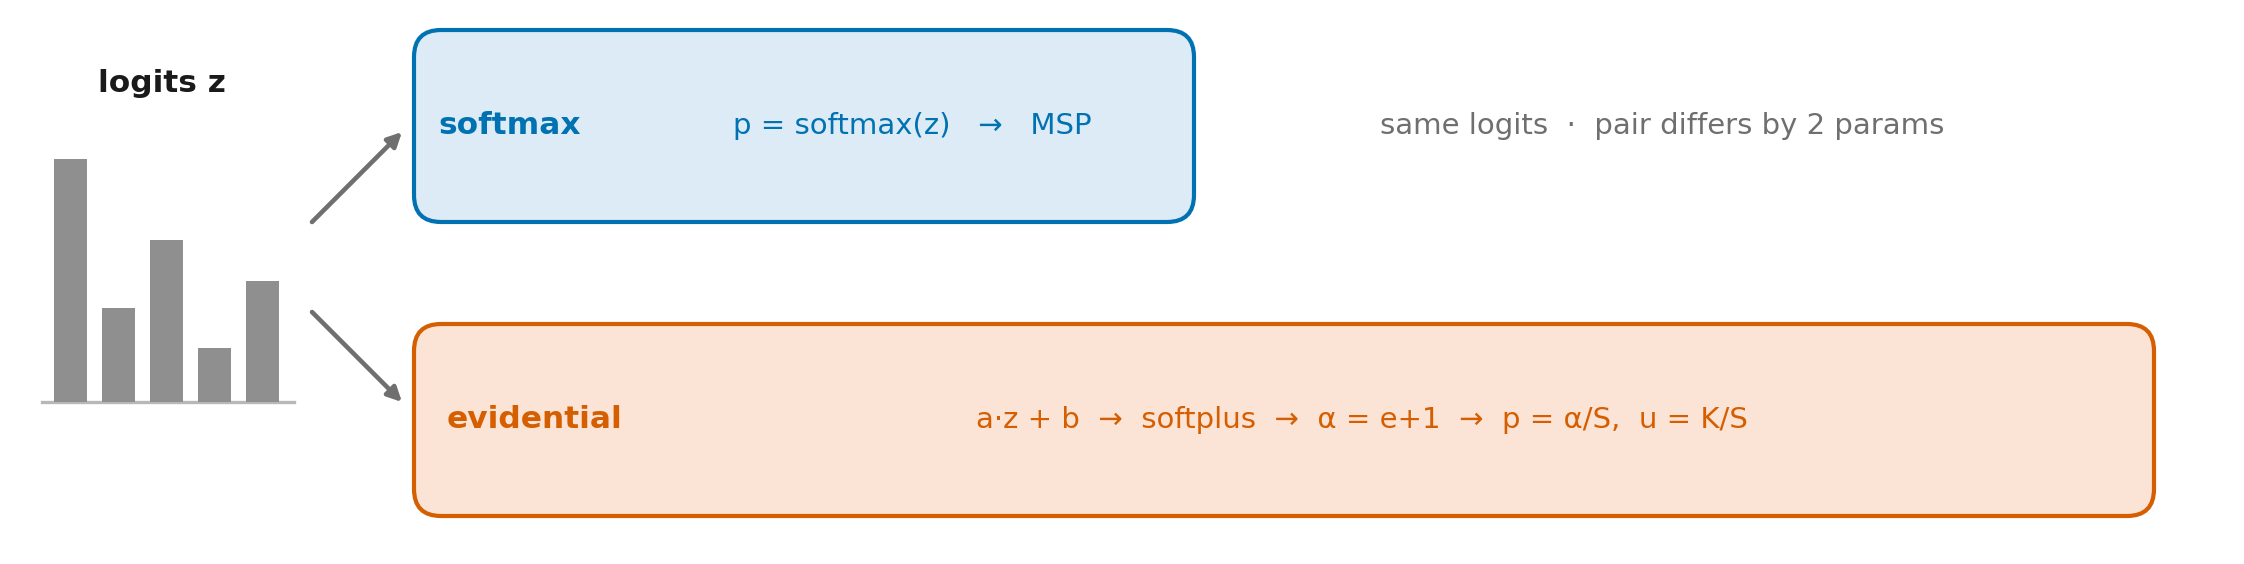
\includegraphics[width=0.95\textwidth]{F6a_head_two_readouts.png}
\caption{One set of logits, read two ways: as softmax probabilities, or as Dirichlet evidence with a
vacuity score. The two readouts differ by two parameters.}
\label{fig:readouts}
\end{figure}

\paragraph{Softmax.} The probabilities are $\hat p = \mathrm{softmax}(z)$ and the predicted class is the
arg-max.

\paragraph{Evidential.} Following Sensoy et al.~\cite{sensoy2018edl}, the logits are mapped to
non-negative evidence, which defines a Dirichlet distribution:
\begin{equation}
e_n = \mathrm{softplus}(a\, z_n + b), \quad \alpha_n = e_n + 1, \quad S = \sum_{n} \alpha_n, \quad
\hat p_n = \frac{\alpha_n}{S}, \quad u = \frac{K}{S}.
\label{eq:evidence}
\end{equation}
The vacuity $u$ is close to 1 when the model has almost no evidence for any class and close to 0 when it
has a lot, regardless of which class the evidence favours. The scale $a$ and bias $b$ are the only
parameters this readout adds. They are learned together with the adapter, start at $a = 2$, $b = -6$,
and $a$ is kept positive so that a higher similarity always produces more evidence.

These two parameters exist because of a failure we hit early in the project. In the first version,
softplus was applied directly to squared-distance logits, which are of the order of $-700$ for
ResNet-18 features. Softplus of such values is essentially zero, so every class received no evidence,
the Dirichlet was uniform, accuracy stayed at chance and the gradients vanished. The bias $b$ moves the
logits into the range where softplus responds, and the scale $a$ sets how quickly evidence grows above
that point. The same evidence function is used in the training loss, in evaluation and in OOD scoring,
so the three can never disagree.

\begin{table}[H]
\centering
\caption{The two readouts. Both use the same logits (\cref{eq:logits}).}
\label{tab:readouts}
\begin{adjustbox}{max width=\textwidth}
\begin{tabular}{@{}lll@{}}
\toprule
& Softmax & Evidential (Dirichlet) \\
\midrule
Output & class probabilities & evidence $\rightarrow$ Dirichlet $\rightarrow$ probabilities \\
Native uncertainty score & maximum probability (MSP) & vacuity $u = K/S$ \\
Extra parameters & 0 & 2 (scale $a$, bias $b$) \\
\bottomrule
\end{tabular}
\end{adjustbox}
\end{table}

\section{Training}
\label{sec:training}

\subsection{Losses}
\label{sec:edl-loss}

Softmax models are trained with cross-entropy on the query predictions. Evidential models use the
squared-error loss of Sensoy et al.~\cite{sensoy2018edl} without its variance term, which Chen et
al.~\cite{chen2024redl} found unnecessary and harmful to calibration, plus the usual Kullback--Leibler
penalty on evidence for the wrong classes:
\begin{equation}
\mathcal{L} = \sum_{k=1}^{K} \bigl(y_k - \hat p_k\bigr)^2 + \lambda_t\, \mathrm{KL}\bigl[\mathrm{Dir}(\tilde\alpha)\,\Vert\,\mathrm{Dir}(\mathbf{1})\bigr],
\qquad \tilde\alpha = y + (1 - y) \odot \alpha .
\end{equation}
Removing the correct class's evidence before the KL term means only misleading evidence is pushed toward
the uniform prior. The weight $\lambda_t$ rises linearly from 0 to 0.1 over the first 1,000 training
episodes, so the penalty does not suppress evidence before the model can separate the classes.

\subsection{Episodic training}

The adapter (and, for evidential models, $a$ and $b$) is trained on episodes sampled from the 64
training classes, with the same shot count as at test time. For each episode the support and query
images pass through the backbone and adapter, prototypes are formed, query logits are computed, and the
loss is back-propagated to the trainable parameters only. We use Adam with learning rate
$5 \times 10^{-3}$ and no weight decay, 100 training episodes per epoch and at most 30 epochs. After every
epoch the model is evaluated on the 100 validation episodes; training stops when validation accuracy has
not improved for 5 epochs, and the weights from the best validation epoch are kept. One recipe is used
for every configuration and was not tuned per configuration.

\section{OOD Scoring Rules}
\label{sec:scores}

Four uncertainty scores are compared:
\begin{itemize}
\item \textbf{MSP}~\cite{hendrycks2017baseline}: the largest softmax probability, $\max_n \hat p_n$.
\item \textbf{TS-MSP}: MSP after temperature scaling~\cite{guo2017calibration}, with the temperature fitted
on the validation episodes.
\item \textbf{Energy}~\cite{liu2020energy}: $\log \sum_n \exp(z_n)$, computed directly on the raw logits.
Liu et al.\ define the energy as the negative of this quantity; we use the sign for which a higher value
means more in-distribution. It has no parameters.
\item \textbf{Vacuity}: $u = K/S$ from \cref{eq:evidence}.
\end{itemize}
In the main grid each model is scored with its native readout only: evidential models with vacuity and
softmax models with MSP, TS-MSP and energy. Any comparison between them therefore changes the training
objective and the score at the same time. RQ2 removes this confound by computing all four scores on all
120 models (\cref{sec:rq2}). Energy is computed on the same raw logits for both kinds of model. Vacuity on
a softmax-trained model needs values for $a$ and $b$, which such a model never learned, so for RQ2 we fit
them on the validation episodes with the same procedure for both training objectives (\cref{sec:refit}).

\section{Post-Hoc Refit of the Evidential Head}
\label{sec:refit}

RQ4 asks whether the evidential head's calibration can be improved after training. We keep the backbone,
adapter and prototypes fixed and refit only $a$ and $b$ on the validation-episode logits by minimising the
negative log-likelihood of $\hat p = \alpha / S$ (500 Adam steps, learning rate 0.05). This mirrors
temperature scaling~\cite{guo2017calibration}, which also fits a tiny number of parameters on held-out
data by minimising NLL. There is one important difference. Temperature scaling is a monotone rescaling
of each logit and cannot change the ranking of inputs by confidence. Vacuity, however, depends on the
evidence summed over all five classes, so changing $a$ and $b$ can reorder which images look most
unfamiliar. Whether the OOD ranking survives therefore has to be measured, and RQ4 measures it.

\section{Experimental Design}
\label{sec:design}

\subsection{The main grid}

The main grid crosses five two-level factors in a full factorial design (\cref{fig:design}):
\begin{itemize}
\item dataset: CIFAR-FS or MiniImageNet;
\item shots: 1 or 5;
\item backbone: ResNet-18 or MobileNetV3-Small;
\item adapter: parallel bottleneck or LoRA;
\item head: softmax or evidential.
\end{itemize}
This gives $2^5 = 32$ configurations. The two baselines (full fine-tuning and linear probe, with both
heads and both shot counts, on ResNet-18 and CIFAR-FS) add 8 configurations, for 40 in total. Each is
trained with 3 seeds, giving 120 runs, all evaluated on the same 600 test episodes. The baselines are not
part of the balanced factorial and are left out of the variance decomposition of RQ1.

\begin{figure}[H]
\centering
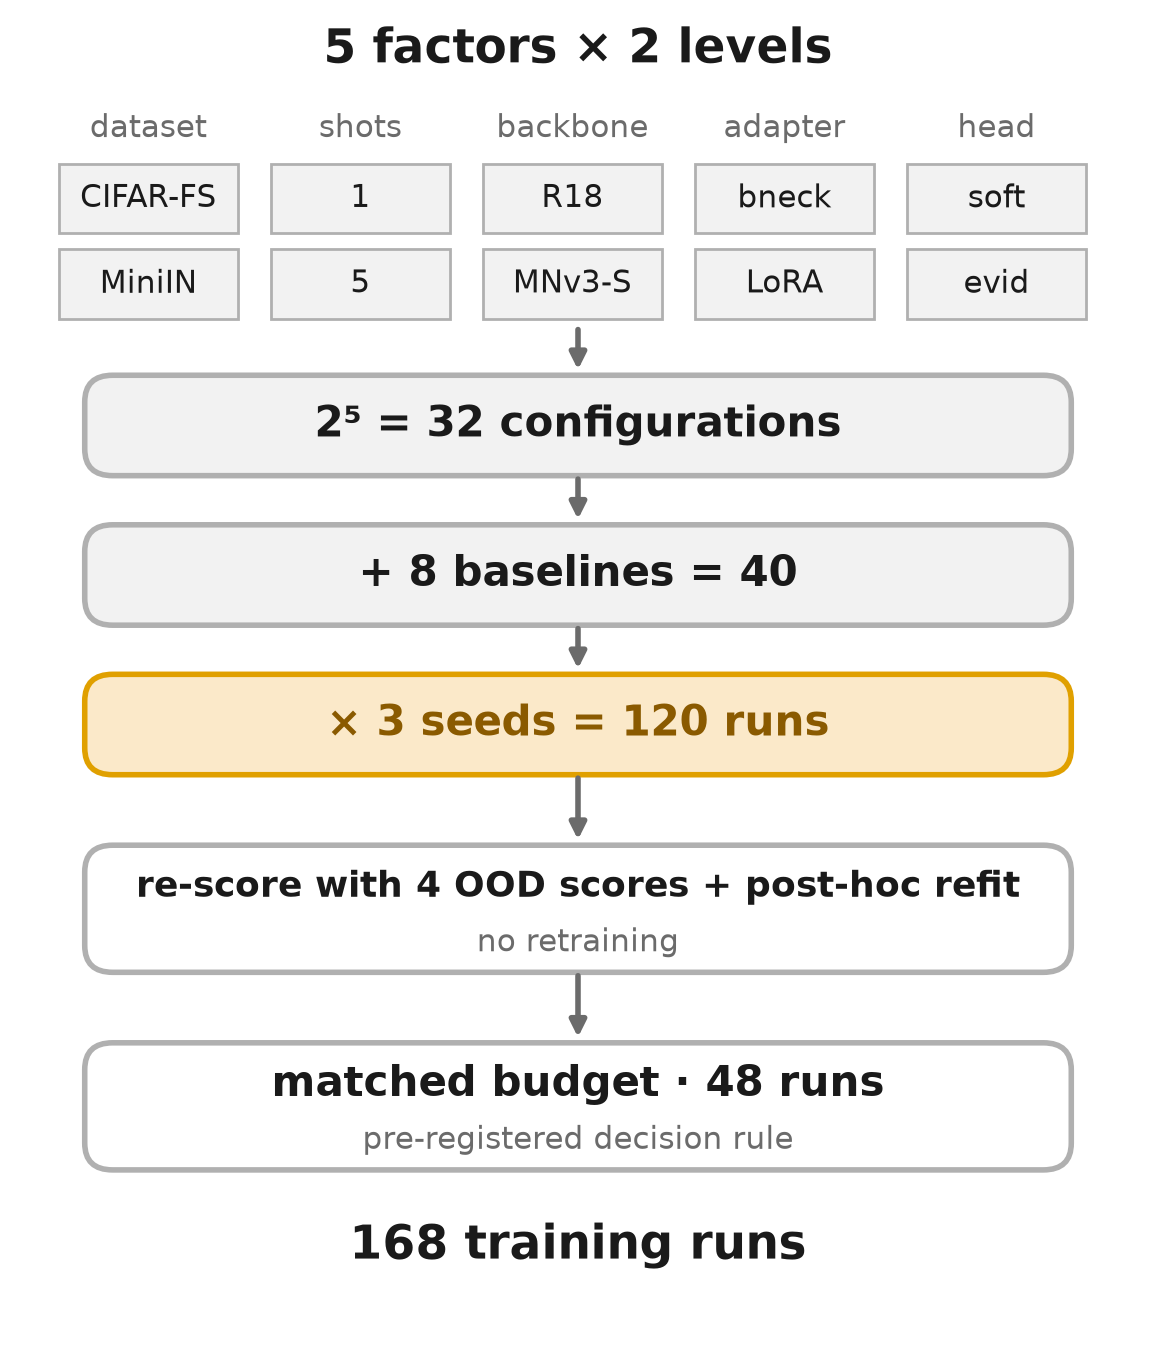
\includegraphics[width=0.55\textwidth]{F7_experimental_design_flow.png}
\caption{The experimental design: the 120-run grid, re-scored with four OOD scores and refitted post hoc
without retraining, followed by the 48-run matched-budget experiment.}
\label{fig:design}
\end{figure}

A structural feature of this grid makes RQ3 possible. Because the bottleneck adapter's size depends on
the channel widths of all four stages while LoRA's depends on one layer, the ordering of the two adapters'
sizes reverses between backbones (\cref{tab:budgets}).

\begin{table}[H]
\centering
\caption{Trainable parameters of the two adapters (softmax head; the evidential head adds 2). The size
ordering reverses between backbones.}
\label{tab:budgets}
\begin{adjustbox}{max width=\textwidth}
\begin{tabular}{@{}lrrl@{}}
\toprule
Backbone & Bottleneck & LoRA & Larger adapter \\
\midrule
ResNet-18 & 31,744 & 12,288 & bottleneck, by $2.58\times$ \\
MobileNetV3-Small & 6,928 & 10,752 & LoRA, by $1.55\times$ \\
\bottomrule
\end{tabular}
\end{adjustbox}
\end{table}

\subsection{The matched-budget experiment}
\label{sec:matched-design}

In the grid the size ordering always flips together with the backbone, so ``the larger adapter is better
calibrated'' and ``the backbone decides which adapter is better calibrated'' predict exactly the same
pattern. To tell them apart we rebuilt both adapters with the \emph{same} number of parameters within each
backbone, at two budget levels per backbone, by changing only the rank (\cref{tab:matched-budgets}). The
experiment uses MiniImageNet 5-shot, both heads (trained separately) and 3 seeds: 2 backbones $\times$ 2
levels $\times$ 2 adapters $\times$ 2 heads $\times$ 3 seeds = 48 runs, 18 of which repeat grid
configurations and reproduced the grid's numbers exactly. On MobileNetV3-Small the high level is 9.4K
rather than 10.8K because the bottleneck rank cannot exceed the 24 channels of the shallowest stage.

\begin{table}[H]
\centering
\caption{Matched budgets (softmax head). The two adapters differ in size by at most 3.1\%, against 55--158\%
in the grid.}
\label{tab:matched-budgets}
\begin{adjustbox}{max width=\textwidth}
\begin{tabular}{@{}llrrr@{}}
\toprule
Backbone & Level & Bottleneck (rank $\rightarrow$ params) & LoRA (rank $\rightarrow$ params) & Difference \\
\midrule
ResNet-18 & low & 6 $\rightarrow$ 12,504 & 16 $\rightarrow$ 12,288 & 1.8\% \\
ResNet-18 & high & 16 $\rightarrow$ 31,744 & 41 $\rightarrow$ 31,488 & 0.8\% \\
MobileNetV3-S & low & 16 $\rightarrow$ 6,928 & 10 $\rightarrow$ 6,720 & 3.1\% \\
MobileNetV3-S & high & 22 $\rightarrow$ 9,448 & 14 $\rightarrow$ 9,408 & 0.4\% \\
\bottomrule
\end{tabular}
\end{adjustbox}
\end{table}

The decision rule was written down and committed before any of these runs existed. The analysis unit is
a backbone $\times$ head cell (four cells), averaging its two budget levels. Let $\Delta$ be LoRA's ECE minus
the bottleneck's, and $\sigma$ the pooled across-seed standard deviation of the two adapters,
$\sigma = \sqrt{(s_{\text{btl}}^2 + s_{\text{LoRA}}^2)/2}$, with sample standard deviations over the
three seeds. The hypotheses and their pre-registered criteria were:
\begin{itemize}
\item \textbf{Budget:} the gap collapses once budgets are equal. The matched $|\Delta|$ is at most half of
the unmatched $|\Delta|$ (collapse ratio $\le 0.5$) and lies within $2\sigma$ of zero.
\item \textbf{Architecture:} one adapter is better calibrated on both backbones. The matched $\Delta$ has the
same sign on both backbones and exceeds $2\sigma$.
\item \textbf{Backbone:} the per-backbone signs of the grid survive at equal budget. The matched $\Delta$
keeps its unmatched sign (positive on ResNet-18, negative on MobileNetV3-Small) and exceeds $2\sigma$.
\end{itemize}
A hypothesis is supported if its rule fires in at least 3 of the 4 cells; if none does, the result is
recorded as inconclusive.

\section{Implementation}

The code is written in PyTorch and driven by configuration files, so that each experiment states only
how it differs from a shared base configuration. Every run seeds Python, NumPy and PyTorch and uses
deterministic cuDNN kernels; evaluating the same checkpoint twice gives byte-identical result files.
Training ran on NVIDIA Tesla T4 GPUs on Google Colab and Kaggle.
